\documentclass[12pt,a4paper]{report}
\synctex=1
\usepackage[utf8]{inputenc}
\usepackage[margin=2cm, top=1.5cm, bottom=2cm]{geometry}
\usepackage{graphicx}
\usepackage{libertine}
\usepackage{amsmath}
\usepackage{amssymb}
\usepackage{listings}
\usepackage{pgfornament}
\usepackage{eso-pic}
\usepackage{textcomp}
\usepackage{courier}
\usepackage[hangul]{kotex}
\usepackage{rotating}
\usepackage{dirtree}
\title{
	\centering
	\pgfornament[width=12cm,color=teal]{84}\\
	\vspace{1cm}
	\fontsize{50}{50} \selectfont {설계과제 최종 보고서\\예약 시스템 구현}\\
		\pgfornament[width=12cm,color=teal]{88}\\
	\vfill}
\author{
	\LARGE
	\begin{tabular}{rl}
		\hline
		교과목명 : & 자료구조와 실습\\
		담당교수 : & 정 준호 교수님\\
		학과 : & 불교학부 \\
		학번 : & 2016110056\\ 
		이름 : & 박승원\\
		날짜 : & \today\\
		\hline
	\end{tabular}\vspace{2cm}
	\\

\includegraphics[width=0.5\textwidth]{logo.jpg}
	}
\date{}


\linespread{1.3}

\begin{document}

\maketitle

%\includegrap

\newpage
\tableofcontents
\newpage
\chapter*{과제 요약서}
\paragraph{설계 과제명} 예약 시스템 구현\\ 
\paragraph{주요기술용어} 단일 연결 List, TCPIP, 모듈화\\
\paragraph{1. 과제목표} 자신에 맞게 customize 할 수 있는 범용의 예약 프로그램\\
\paragraph{2. 수행 내용 및 방법} C, C++, TCPIP, GTKmm등을 이용하여 Makefile 프로젝트로  프로그램 작성\\
\paragraph{	3. 수행 결과} TCPIP환경에서 사용할 수 있으며, 그래픽 환경을 갖춘 예약 프로그램을 완성하였다. 안정성과 보안이 크게 중요하지 않은 경우라면 얼마든지 개인 사업자들이 사용할 수 있을 정도의 품질이라고 생각된다.\\
\paragraph{	4. 결과 분석} 개발자의 측면에서는 리스트 자료구조를 활용하여 사용자 편의성과 소스 재사용성을 높인 프로그램을 만들었다.\\

\noindent
\chapter{서론}
\section{설계과제 목적}
예약 시스템을 구축하기 위하여 필요한 여러 가지 자료, 즉 예약 입력, 예약조회, 예약삭제 등의 자료구조를 리스트 형태로 설계하고 이를 운영하는 함수들을 설계 구현한다.
\begin{itemize}
\item 창의적 사고 및 다양한 방법을 통한 문제 해결 능력
\item 여러 가지 제약조건을 고려한 효율적인 프로그램 설계 능력
\end{itemize}
\section{설계과제 내용}
\subsection{설계과제 내용}
소형의 개인 사업자들이 하나의 컴퓨터로 혹은 공유기, 인트라넷을 기반으로 한 내부 망을 갖춘 영업 환경에서 범용으로 사용할 수 있는 예약 프로그램.

일반적으로 대형 업체들은 자신들의 예약 프로그램을 자신의 목적에 특화시켜서 구현한 것으로, 인터넷 예약, 결제 기능까지 갖추어서 사용할 수 있을 것이지만, 개인 사업자들의 경우는 그럴 만한 투자 여력이 없다. 이러한 개인 사업자들이 사용할 수 있는 범용의 예약 프로그램을 만들어 보고자 한다.

범용의 무료 프로그램이기에 개인사업자들의 각각의 요구에 맞춰 특화된 프로그램을 만들수는 없겠지만, 시설과 예약 시간이라는 두 가지의 추상적인 데이터만으로도 일반적인 모든 경우에 모두 대처할 수 있었다.

여기에서 시설이라 함은 식당인 경우 각각의 테이블이 하나의 시설이 되고, 숙박업소 등에서는 각각의 방이 하나의 시설이 된다.

\subsection{설계/구현 과정}
TCPIP 모듈은 기존의 것을 약간 수정하여야 했다. 리스트 자료구조와 C언어 함수를 활용하기 위해 wrapper 클래스를 작성해야 했다. 프로그램 작성 및 테스트는 생각보다 일찍 끝낼 수 있었다.
\chapter{프로그램의 구조 및 구성}
\section{전체 구성도}
\begin{sidewaysfigure}
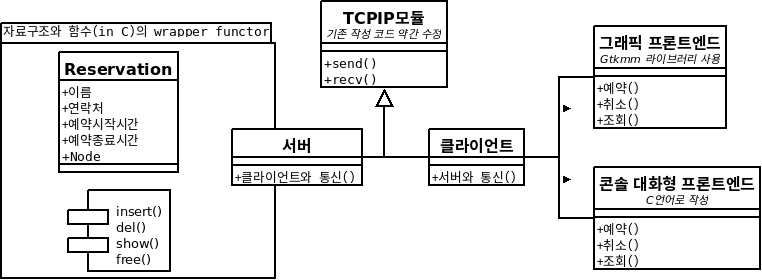
\includegraphics[width = \textwidth]{final2.png}
\caption{호환성을 높이기 위해 프론트엔드를 이용한 서버 클라이언트 모델 예약 시스템 구조}
\label{fig}
\end{sidewaysfigure}

최종 구현물은 다음 페이지의 그림 \ref{fig}와 같이 구현 되었다.
server, client, graphic frontend, console front end의 네 개의 실행화일로 구성된다.

주로 C와 C++을 이용하여 구현하였다.
자료구조와 자료구조를 다루는 함수, 대화형 프론트 엔드 등은 C로 구현이 가능하였으나, TCPIP모듈의 사용과 그래픽 모듈의 사용을 위해서는 부득이하게 C++을 사용할 수 밖에 없었다.
GNU g++과 Makefile을 사용하여 우분투 16.04에서 컴파일했다. 
C와 C++이 매우 간단하게 링크되고 실행이 되었다.
C++이 C를 거의 완벽히 지원하고 있음을 알 수 있었다.
\subsection{TCPIP 모듈}
TCPIP모듈은 선수과목 인정 신청서에 낸 TCPIP 모듈을 약간 고쳐서 사용했다. 
멀티프로세스를 없애고 접속을 유지하지 않는 방식으로 버그를 없애고, 안정화시키는 쪽을 선택했다.
TCPIP 접속을 유지하는 것이 아니라, 문자열을 보내고는 답신을 받는 것으로 종료하는 일회성이므로, 멀티프로세스 없이 TCPIP고유의 큐만으로 처리가 가능하다.
이 모듈이 펑크터를 받아서 서버를 운영하기에 그림 \ref{fig}에서 보는 바와 같이 C함수를 
wrapping하는 클래스를 사용해야 했다.

클라이언트 프로그램은 프론트엔드가 프로그램 내부에서 사용하는 프로그램으로 만들었으나, 독립적으로도 사용이 가능하다.
\subsection{그래픽 프론트 엔드}
그래픽 모듈은 GTKmm을 사용했다. 
Gimp Toolkit은 매우 다재다능한 그래픽 툴킷으로 호환성은 Java나 Qt등에 비해 약간 떨어지나 C++ 고유의 문법을 활용할 수 있는 좋은 도구이다.
우분투 리눅스에서 컴파일하여 실행 확인해 보았다.
\footnote{윈도우 상에서도 컴파일이 가능하다.}

툴킷의 다이얼로그 클래스를 활용하였다.
최대한 문제를 단순화시키기 위해 다이얼로그를 여러 번 부르는 방식으로 구현했다.
다이얼로그는 버튼들을 가지고 있고, 이 버튼들의 크기를 조절하는 식으로 예약시간의 장단을 나타냈다.
또한, 범용 예약 시스템이기에 필수적인 일단위, 혹은 시간 단위로 스케일을 변경해가며 테이블을 나타낼 수 있게 구현하였다.(그림 \ref{gf})
빈 칸을 클릭하면 예약메뉴(그림 \ref{re})를 띄우고, 예약된 칸을 클릭하면 취소 메뉴를 띄우는 식으로 직관적인 인터페이스를 사용하였다.

\begin{figure}
	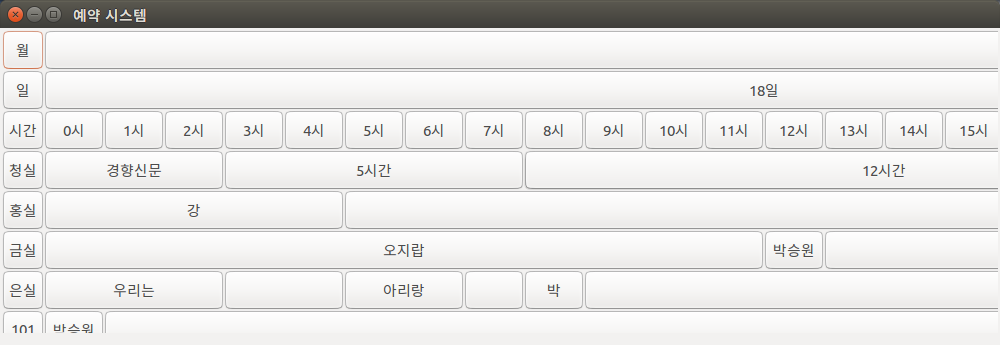
\includegraphics[width=\textwidth]{exec.png}
	\caption{프론트 엔드 메인 화면}\label{gf}
\end{figure}

\begin{figure}
	\centering
	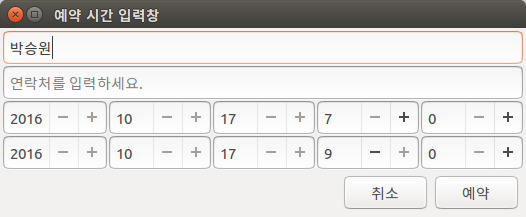
\includegraphics[width=0.7\textwidth]{reser.png}
	\caption{예약 메뉴}\label{re}
\end{figure}
\subsection{콘솔 대화형 프론트 엔드}
호환성이 가장 좋은 것은 뭐니뭐니해도 콘솔이므로, 콘솔에서 대화형으로 예약과 취소를 하는 프로그램도 만들었다.(그림 \ref{con}) 
시간의 입력을 편하게 하기 위해 현재 시간을 디폴트로 할 수 있게 하여, 엔터키만 두드리는 것으로 입력가능하게 하였다.

\begin{figure}
	\centering
	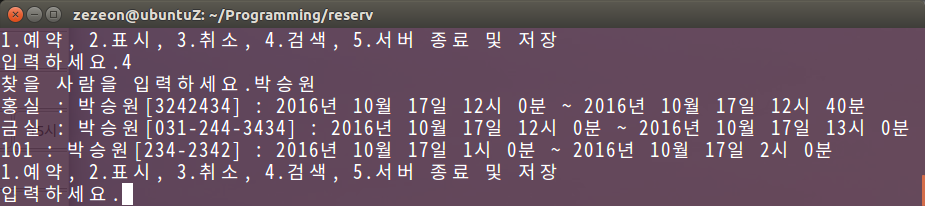
\includegraphics[width=\textwidth]{con.png}
	\caption{콘솔 프론트 엔드}\label{con}
\end{figure}

\section{프로그램 세부 구성}
\subsection{Tree 구조와 파일}

\dirtree {%
.1 root.
.3 Makefile : 하위 디렉토리의 Makefile들을 실행시킴.
.3 serverip.cfg : 클라이언트가 서버의 IP주소를 찾을 파일.
.3 facility.txt : 자신의 업체의 시설 상황 파일.
.2 src. 
.3 Makefile.
.3 server.cpp.
.3 client.cpp.
.3 console\_front.cpp.
.3 tcpip.cc : TCPIP 모듈.
.3 tcpip.h.
.3 reserv.cc : wrapper class.
.3 reserv.h.
.3 reser.cc : C언어, List를 사용한 자료구조와 함수.
.2 gtk.
.3 Makefile.
.3 frontend.cc.
.3 frontend.cpp.
.3 frontend.h.
.2 OBJ.
.3 Makefile : obj파일들을 링크하는 역할.	
}

소오스의 트리 구조는 위와 같다. 
gtk에는 GTKmm 라이브러리를 쓰는 소스들이 들어있고, src에는 그 외의 모든 소스들이 있다. 
OBJ에는 소스를 컴파일한 목적파일들이 들어갈 장소이다.
루트 디렉토리에 있는 Makefile은 src, gtk, OBJ의 순으로 각 하위 디렉토리의 Makefile을 실행시킨다.

확장자 cpp인 파일들은 실행화일이 될 main함수가 들어간 소오스이다.
확장자 cc인 파일들은 목적파일로 만들어질 구현부이다.
Makefile 작성의 편의를 위해 C언어 소스도 cc로 확장자를 정했다.

root 디렉토리에서 make을 한 번만 실행시키면 루트 디렉토리에 모든 실행파일이 만들어진다.

\subsection{Source 설명}
\lstinputlisting[frame=single,language=C++,columns=flexible,caption={reserv.h :\quad List자료구조, 함수, 랩퍼 클래스를 모두 기술한 헤더 파일},basicstyle=\normalsize]{src/reserv.h}

위의 헤더 파일은 이 프로젝트에서 가장 핵심적인 ADT라고도 할 수 있으므로, 이에 대해 설명한다.
우선 시간을 2000년을 0값으로 한 int값으로 단순화하여 프로그래밍의 편의를 도모하였다.
그로 인해 time 구조체를 위의 int값으로 바꾸어주는 함수와 그 역을 행하는 함수
\footnote{to\_time()과 to\_minute()함수}
를 따로 작성했다.
리스트는 단일연결 리스트로 만들었다. 
리스트에 삽입 및 삭제, 보기 하는 함수들은 모두 C로 작성하였으며, wrapper class에서는 이 함수들을 단순히 부른다.
\footnote{각 함수의 주석을 보십시오.}
원래의 계획안과 약간 달라진 것은 시설물들의 리스트를 만드는 것인데, 예약시간은 리스트를 이용하기로 하고, 시설물은 map을 이용하기로 변경하였다.
그로 인해, 예약 시설물의 이름만으로 리스트의 포인터를 찾아오기가 편해졌다.
그 이외의 상세한 내용은 소스 파일을 참고하기를 바랍니다.
\chapter{결과 및 토의}
\section{프로그램 테스트 결과}
\begin{sidewaysfigure}
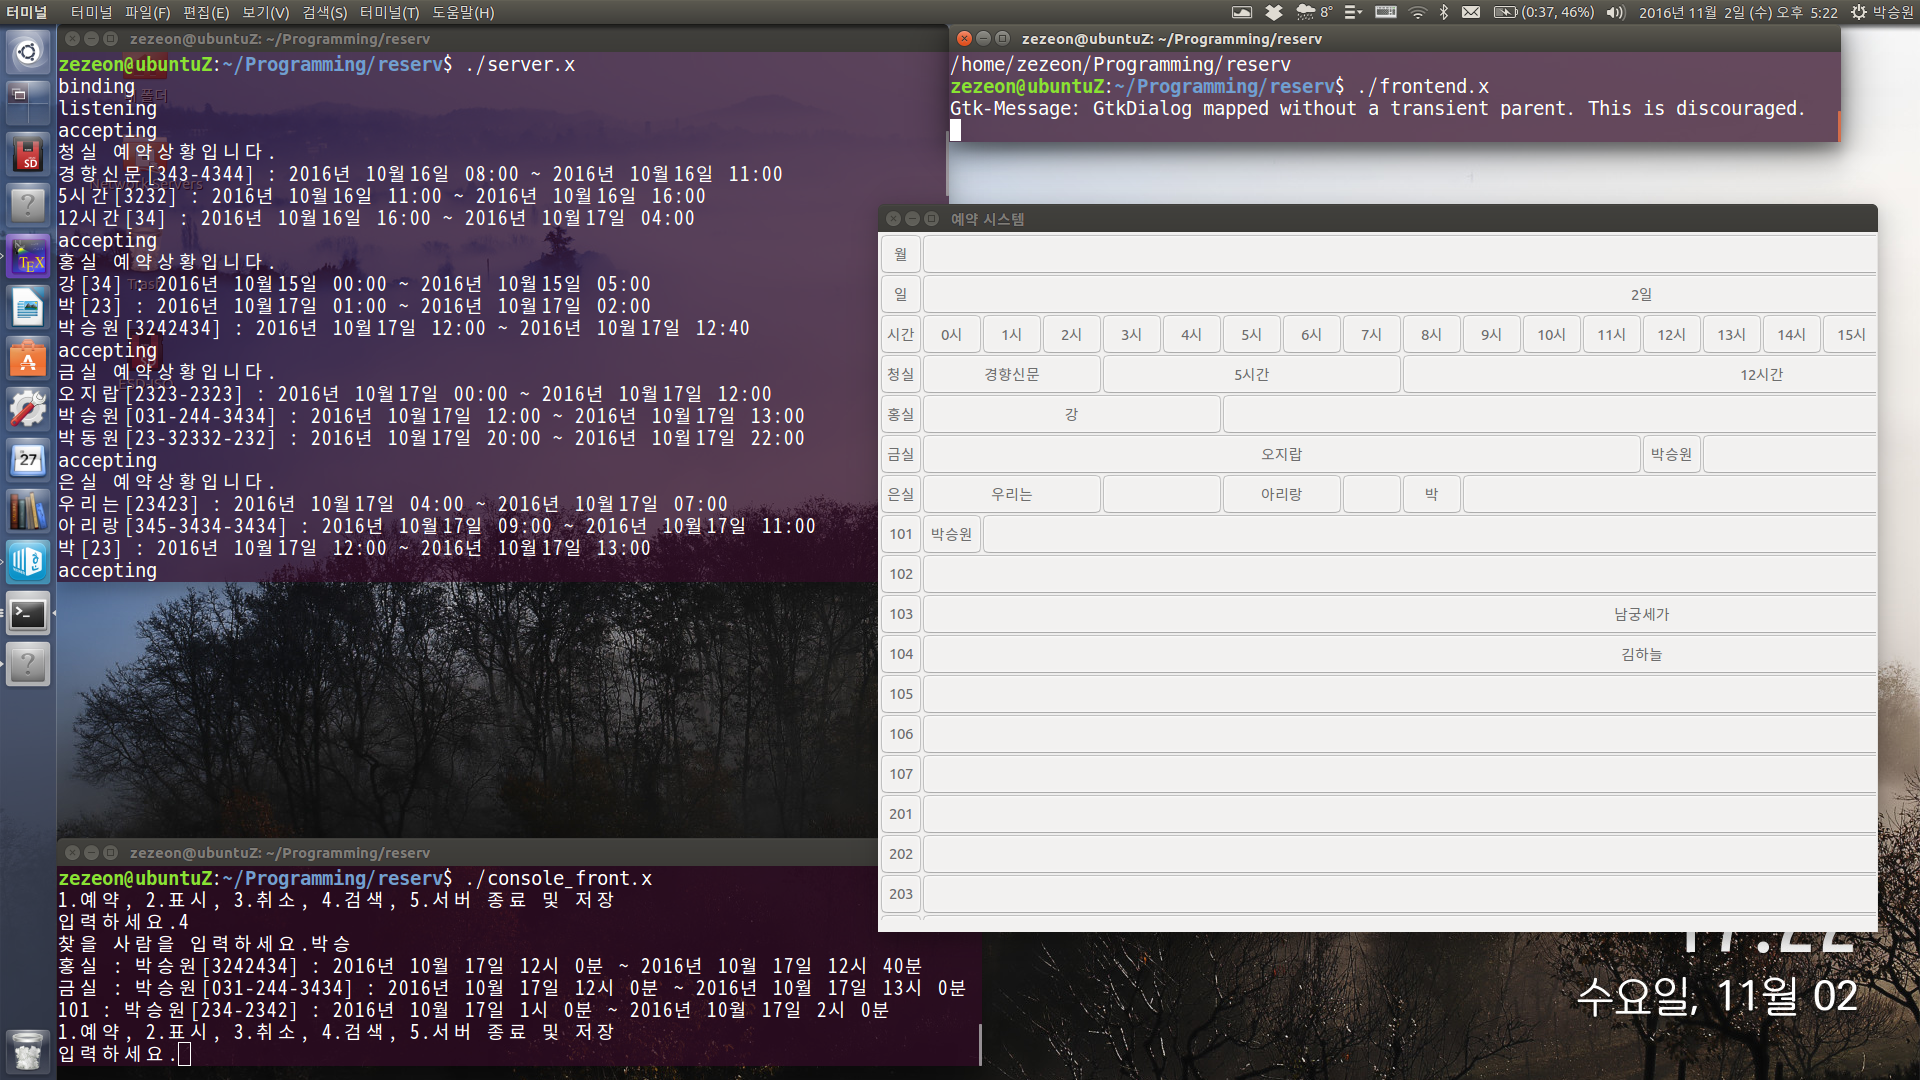
\includegraphics[width=\textheight]{screen.png}
\caption{다중 접속 중인 프로그램 실행 화면}
\label{exe}
\end{sidewaysfigure}
그림 \ref{exe}에서 좌상단의 터미널에서는 서버를 실행했고, 우상단의 터미널과 그래픽 프로그램은 그래픽 프론트엔드를 실행했으며, 좌하단의 터미널에서는 콘솔 프론트 엔드를 실행했다.

동시에 서버에 접근하는 데에 문제가 없이 TCPIP환경을 최대한 활용하고 있음을 확인할 수 있었다.
그 외에 예약이나, 취소, 조회 등의 기능도 모두 잘 작동되었다.
본 프로그램은 GKTmm을 제외하면 표준 라이브러리만을 사용하였기 때문에, 다른 운영체제에서도 잘 컴파일이 되리라 생각된다.
\section{기타}
과제 제출이 마감에 가까워서야 가능한데, 최종 보고서의 형식을 미리 알 수 있도록 과제 제출을 프로젝트 수행 시작하면서 가능하도록 해주시면 감사하겠습니다.

\chapter{부록}
매뉴얼 : 별첨\\ 소스코드 : 별첨
\end{document}
